\documentclass[letterpaper, 12pt]{article}

\usepackage[normalem]{ulem}
\usepackage{scrextend}	% for the indented environment
\usepackage{amsmath,amsthm,amssymb,amsfonts}
\usepackage{graphicx, caption, subcaption}
\usepackage{hyperref}
\usepackage[top=1in, bottom=1in, left=1in, right=1in]{geometry}

\newcommand{\figurepath}{../../Figures}

% make everything 12pt font
\let\Huge\normalsize
\let\huge\normalsize
\let\LARGE\normalsize
\let\Large\normalsize
\let\large\normalsize
\let\small\normalsize
\let\footnotesize\normalsize
\let\scriptsize\normalsize
\let\tiny\normalsize

% Make everything single spacing
\linespread{1.0}

\begin{document}
%Header-Make sure you update this information!!!!
\noindent
\textbf{Study and Comparison of the Neuroidal Model} \hfill \newline Cathy Chen and Stefan Keselj \\
COS511 Final Project Report \\
Due May 15, 2018\newline

* For page limit purposes, we uploaded report\_separatefigures.pdf with all figures moved to the end of the report.

\section{Introduction}
For our project we chose to study a new topic, a biologically plausible model of learning proposed by Les Valiant in 1994 \cite{valiant_circuits_1994}. We mainly studied Valiant's book \textit{Circuits of the Mind} and a few follow-up papers from Valiant and Papadimitriou \& Vempala. In this report we present a concise summary of our study (describing the model, relevant algorithms, and methods of analysis) and we implement and simulate two learning algorithms on this model. We then compare this model to hypotheses about the human brain and to modern artificial neural networks.

\section{Neuroidal Model}\label{sec:model}
We summarize our understanding of the neuroidal model, primarily drawing from \cite{valiant_circuits_1994, valiant_memorization_2005, papadimitriou_cortical_2015}.

The neuroidal model consists of a system of \underline{neurons} and \underline{synapses} which can be modeled as a weighted directed graph in which nodes represent neurons and edges represent synapses. Each neuron $i$ has a state $s_i$ containing three variables: a threshold $T\in\mathbb{R}_{>0}$, a categorical memory variable $q$, and an indicator variable $f$ that indicates whether the network is firing. (In more complex versions of the model, $T\in\mathbb{R}^\gamma$, for $\gamma\in\mathbb{Z}$, which allows each neuron to store multiple pieces of information in memory.) The synapse from neuron $i$ to neuron $j$ is represented by $w_{ji}\in W$, where $W$ may be a set such as $\mathbb{R}$ or $\{0,1\}$. In some versions of the model, each synapse also contains a memory state $qq$. The network represents each conceptual \underline{item} by a randomly selected set of $r$ neurons, as we show in Figure \ref{fig:itemrepresentation}. The activation of an item (the system ``thinking about" the item) is represented by the item's nodes firing.

\begin{figure}[!htb]
\centering
\begin{subfigure}[b]{0.45\textwidth}
      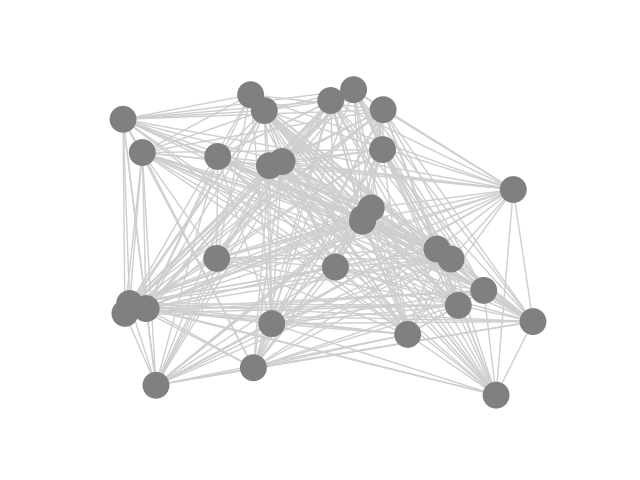
\includegraphics[width=\textwidth]{\figurepath/initialmodel.png}
      \caption*{Randomly initialized network.}
\end{subfigure}
\begin{subfigure}[b]{0.45\textwidth}
      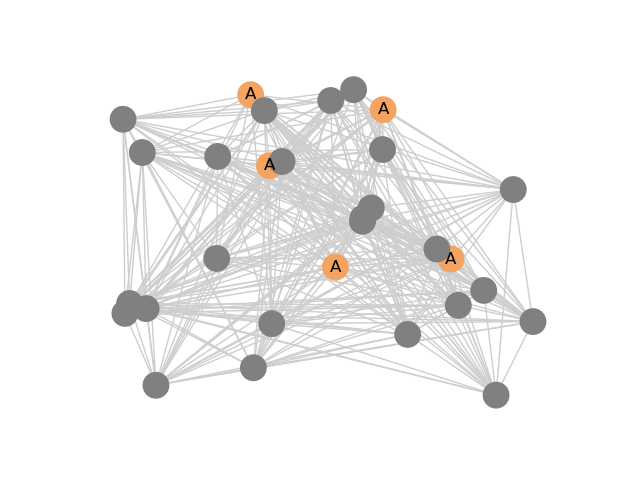
\includegraphics[width=\textwidth]{\figurepath/itemrepresentation.png}
      \caption*{$r$ neurons represent item $A$.}
\end{subfigure}
\caption{Item representation in a neuroidal network.}
\label{fig:itemrepresentation}
\end{figure}

The system operates with discrete timesteps and all neuroid and synapse states update at each timestep according to predefined functions. The functions have the form $s_{i,t+1}=\delta(s_{i,t},w_i)$, $w_{ji,t+1}=\lambda(s_i,w_i,w_{ji},f_j)$, where $w_i$ is the sum over all $w_{ki}$ for all firing neurons $k$. In particular, neuron firing updates according to the following rule: neuron $i$ fires for a pre-determined number of timesteps if $w_i>T$. In some models, a neuron may be unable to fire for a certain number of timesteps after firing. These functions are local and are part of \underline{vicinal} algorithms: each neuron's update depends only on its own state, the weights connecting the neuron and its neighbors, and the neighbors' firing. 

In \cite{valiant_circuits_1994} Valiant describes two dichotomies of learning: one between memorization (storing explicitly provided or logically deduced information) and inductive learning (acquiring knowledge more general than the explicitly provided examples), and the other between supervised (learning from labeled examples) and unsupervised (learning from unlabeled examples) learning. He notes that the example-based learning and PAC learning framework that we studied in COS511 fall into supervised inductive learning. These dichotomies produce four modes of learning, and Valiant presents algorithms that perform all four modes of learning in the neuroidal model. He constructs algorithms that allow a neuroidal network to recognize a previously presented input (unsupervised memorization), associate two items (supervised memorization), learn functions of a particular class based on a set of provided examples (supervised inductive learning), and learn statistical correlations from a set of provided examples (unsupervised inductive learning).

In addition to neurons and synapses, a learning system can use various \underline{peripherals} to perceive and attend to various items, store intermediate information, and organize the longer-scale timing needed in various algorithms. Valiant suggests that the combination of peripherals and knowledge gained through memorization and inductive learning could allow for higher-level reasoning.

\section{Selected Algorithms}\label{sec:selected_algorithms}
We chose to focus on the $JOIN$ and $LINK$ functions, which (in terms of Valiant's dichotomies) perform unsupervised and supervised memorization  and (in terms of cognitive functions) form memories and associations \cite{valiant_circuits_1994, papadimitriou_cortical_2015}. We provide a high-level overview of these functions and our implementation, and describe an extension of $JOIN$ and $LINK$ proposed by Papadimitriou \& Vempala.

The algorithms for these functions assume that networks have two modes, a ``learning" mode in which the network stores knowledge by updating synapses, and an ``execution" mode in which networks draw upon previously stored knowledge. In the execution modes neuron firing passes through synapses and neurons fire if their total incoming firing falls above some threshold, as we describe in Section \ref{sec:model}.

The algorithms to learn both functions take as input two items, which we refer to as ``$A$" and ``$B$".

$JOIN(A,B)$ learns a conjunction of $A$ and $B$. In the learning mode, the network creates a new item ``$C$" that represents the conjunction of $A$ and $B$ and updates synapses accordingly. Then, in the execution mode the network's representation of $C$ will fire whenever the network's representations of $A$ and $B$ fire. For instance, if $A$ represents that item ``ice" and $B$ represents the item ``cream" then $C$ would represent the item ``ice cream". Seeing ``ice" and ``cream" together would activate the representation of the thought ``ice cream" (rather than the separate thoughts ``ice" and ``cream").

$LINK(A,B)$ learns an association of $A$ and $B$. In the learning mode, $LINK(A,B)$ updates synaptic connections between $A$, $B$, and a set of \underline{relay neurons} which act as an intermediary between the two items. Then, in the execution mode the item $B$ will activate in response to the activation of $A$. For instance, if $A$ represents the idea ``bell" and $B$ represents the idea ``food", then $LINK(A,B)$ would form an association in which the thinking about ``bell" will induce thoughts about ``food".

\subsection{Implementation and Simulation}
We implement the neuroidal model and algorithms that learn the $JOIN$ and $LINK$ functions according to descriptions in \cite{valiant_memorization_2005}. We provide our implementation, additional details, and pseudocode for learning algorithms on \href{https://github.com/cchen23/neuroidal_model_project/tree/master/Code}{github}.

We simulate these algorithms on neuroidal networks with $n$ total neurons. Each time we create a new item, the network sets $r$ randomly chosen neurons to represent the item. (In the simulations we show items do not share neurons, but this is not necessary.) We choose a firing threshold $T=100$ for each neuron, initialize the network so that each pair of neurons has probability $p$ of being connected with strength $1.0$ and probability $1-p$ of not being connected, and constrain the network to have maximum synaptic strength $\frac{T}{k}$. In our visualizations edge darkness denotes synaptic strengths, a yellow outline denotes a firing neuron, and node are colored according to the items they represent (grey nodes are not assigned to any items).

In Figure \ref{fig:learningJOIN} we show the synaptic updates that occur after a network learns $JOIN(A,B)$. The network allocates a set of nodes for $C$ and updates synaptic weights so that, as we show in Figure \ref{fig:executingJOIN}, in the execution mode $C$ fires in response to the activation of both $A$ and $B$.

\begin{figure}[!htb]
\centering
\begin{subfigure}[b]{0.45\textwidth}
      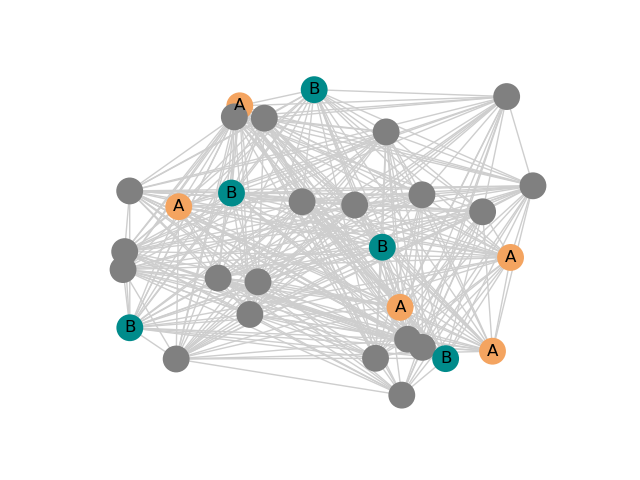
\includegraphics[width=\textwidth]{\figurepath/beforeJOIN.png}
      \caption*{Network before learning $JOIN(A,B)$}
\end{subfigure}
\begin{subfigure}[b]{0.45\textwidth}
      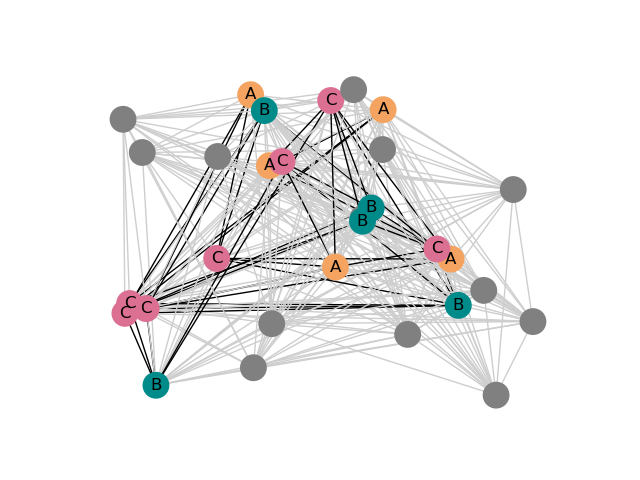
\includegraphics[width=\textwidth]{\figurepath/afterJOIN.png}
      \caption*{Network after learning $JOIN(A,B)$}
\end{subfigure}
\caption{Learning $JOIN(A,B)$ on network with $n=30,p=\frac{1}{2},k=3,r=5$. The network updates synapses from $A$ and $B$ to a set of neurons, $C$, representing $JOIN(A,B)$.}\label{fig:learningJOIN}
\end{figure}

\begin{figure}[!htb]
\centering
\begin{subfigure}[b]{0.45\textwidth}
      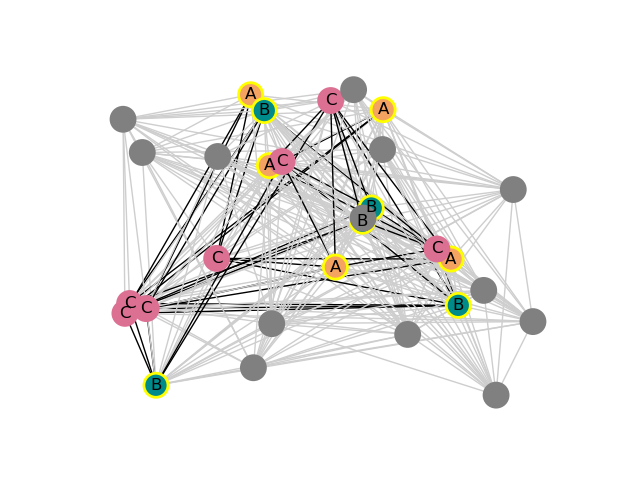
\includegraphics[width=\textwidth]{\figurepath/afterJOIN_fireAB.png}
      \caption*{$t=0$: $A$ and $B$ fire.}
\end{subfigure}
\begin{subfigure}[b]{0.45\textwidth}
      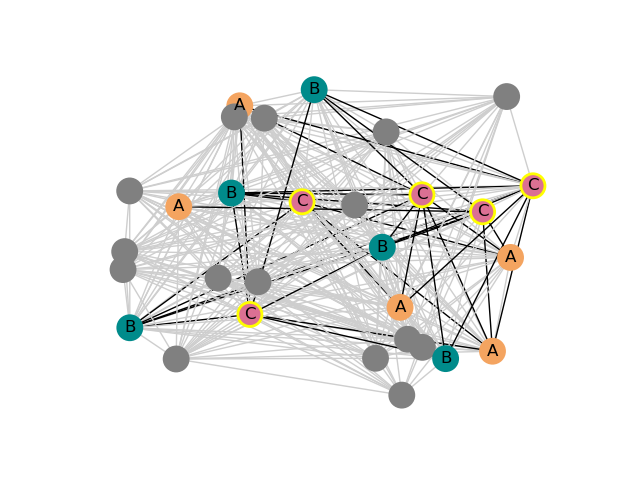
\includegraphics[width=\textwidth]{\figurepath/afterJOIN_fireAB_stepone.png}
      \caption*{$t=1$: $C$ fires.}
\end{subfigure}
\begin{subfigure}[b]{0.45\textwidth}
      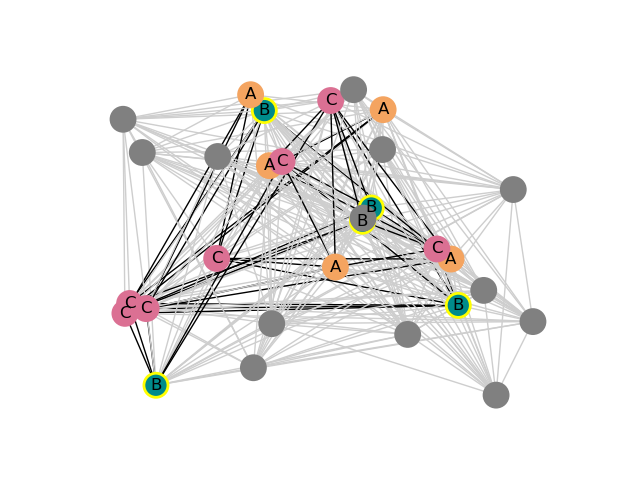
\includegraphics[width=\textwidth]{\figurepath/afterJOIN_fireB.png}
      \caption*{$t=0$: Only $B$ fires.}
\end{subfigure}
\begin{subfigure}[b]{0.45\textwidth}
      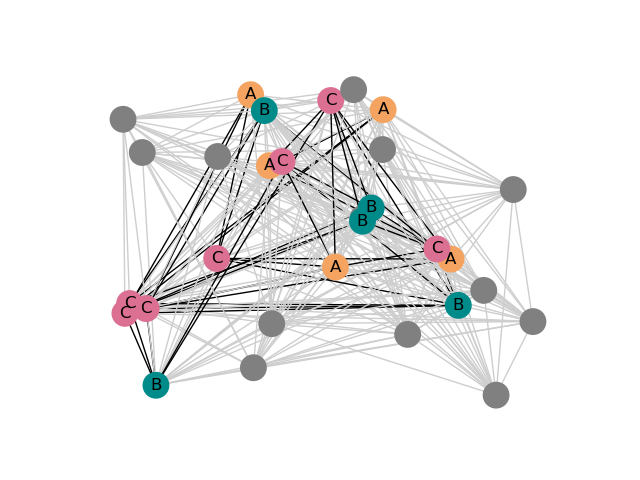
\includegraphics[width=\textwidth]{\figurepath/afterJOIN_fireB_stepone.png}
      \caption*{$t=1$: $C$ does not fire.}
\end{subfigure}
\caption{Executing $JOIN(A,B)$ on network with $n=30,p=\frac{1}{2},k=3,r=5$. $C$ represents the idea $JOIN(A,B)$: it fires if $A$ and $B$ both fire (top panels), but not if only one of $A$ and $B$ fire (bottom panels).}\label{fig:executingJOIN}
\end{figure}

In Figure \ref{fig:learningLINK} we show a network learning $LINK(A,B)$, where it connects $A$ to a set of relay neurons, which in turn are connected to $B$. After learning this function, firing $A$ in the execution mode causes the relay nodes to fire, which then cause $B$ to fire, as we show in Figure \ref{fig:executingLINK}.

\begin{figure}[!htb]
\centering
\begin{subfigure}[b]{0.45\textwidth}
      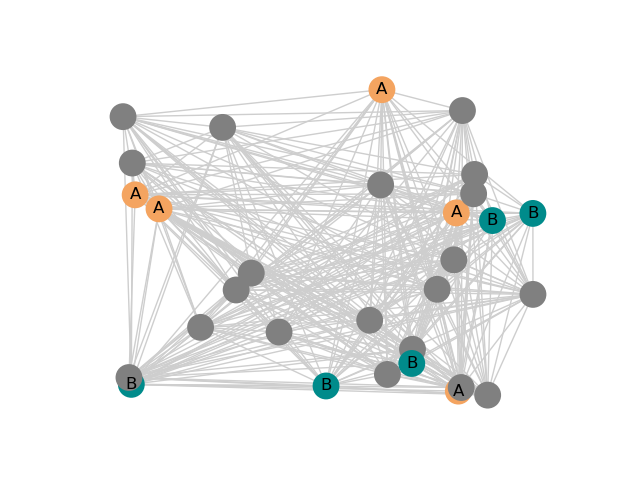
\includegraphics[width=\textwidth]{\figurepath/beforeLINK.png}
      \caption*{Network before learning $LINK(A,B)$}
\end{subfigure}
\begin{subfigure}[b]{0.45\textwidth}
      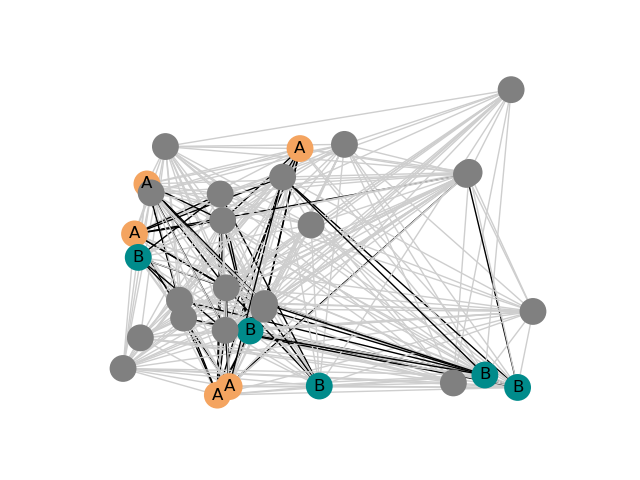
\includegraphics[width=\textwidth]{\figurepath/afterLINK.png}
      \caption*{Network after learning $LINK(A,B)$}
\end{subfigure}
\caption{Learning $LINK(A,B)$ on network with $n=30,p=\frac{1}{3},k=2,r=5$. The network updates synapses from $A$ to a set of relay neurons, and from the relay neurons to $B$.}\label{fig:learningLINK}
\end{figure}

\begin{figure}[!htb]
\centering
\begin{subfigure}[b]{0.3\textwidth}
      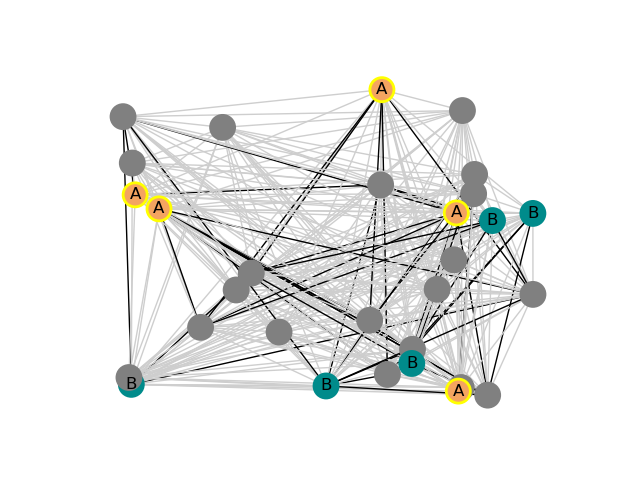
\includegraphics[width=\textwidth]{\figurepath/afterLINK_fireA.png}
      \caption*{$t=0$: $A$ fires.}
\end{subfigure}
\begin{subfigure}[b]{0.3\textwidth}
      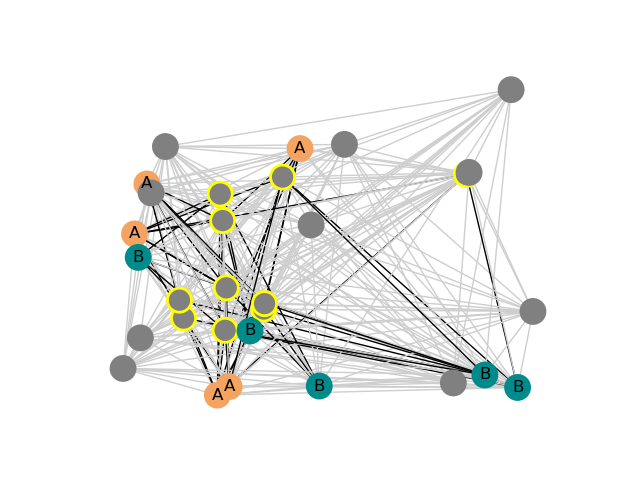
\includegraphics[width=\textwidth]{\figurepath/afterLINK_stepone.png}
      \caption*{$t=1$: Relay neurons fire.}
\end{subfigure}
\begin{subfigure}[b]{0.3\textwidth}
      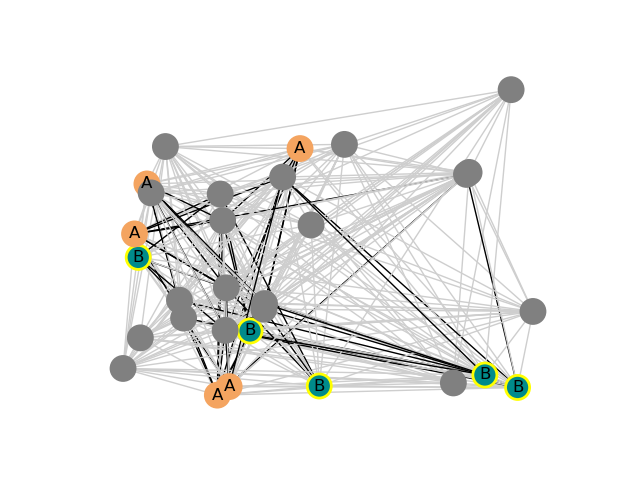
\includegraphics[width=\textwidth]{\figurepath/afterLINK_steptwo.png}
      \caption*{$t=2$: $B$ fires.}
\end{subfigure}
\caption{Executing $LINK(A,B)$ on network with $n=30,p=\frac{1}{3},k=2,r=5$. $A$ firing causes the relay neurons to fire, which in turn cause $B$ to fire.}\label{fig:executingLINK}
\end{figure}

\subsection{Extension by Papadimitriou and Vempala}\label{sec:pjoin}
Papadimitriou and Vempala \cite{papadimitriou_cortical_2015} extend Valiant's $JOIN$ and $LINK$ operations, adding an additional $PJOIN$ operation. The $PJOIN$ operation can memorize $n$-length binary patterns, meaning that it creates an item that fires when the network receives the pattern. Rather than requiring $A$ and $B$ to fire for $C$ to fire (as in the case of $JOIN(A, B)$), after $C$ is created by $PJOIN(A,B)$ if $A$ fires, $C$ will enter a state such that it will fire if only $B$ fires at a later time; Papadimitriou and Vempala refer to this as \underline{mobilizing} $B$. Moreover, this mobilization continues down a chain of $PJOIN$s starting from $B$ and its $PJOIN$ed items. Using this algorithm adds a predictive element to neuroidal model algorithms, allowing efficient memorization of binary patterns. Papadimitriou and Vempala motivate this algorithm by the combinatorial number of $JOIN$s required to solve this memorization task if only the $JOIN$ and $LINK$ functions are used. This inefficiency is especially important since the human brain operates on fast timescales, rendering algorithms requiring more than a small number of steps biologically infeasible.

\subsection{Algorithm Analysis}
Learning algorithms must fulfill certain conditions in order to create useful representations of the desired functions. For $JOIN$, we want it to be highly probable that $C$ (which represents $JOIN(A,B)$ for $r$-item representations of $A$ and $B$) also has $r$ items, that a large majority of the neurons representing $C$ are not active if $A$ and $B$ are not active, and that the representations of $A$ and $B$ only fire if the system is actually thinking of items $A$ and $B$. For $LINK$, we want it to be highly probable that if $A$ is not active then $B$ will not activate, that $B$ will not fire in response to some item with which it is not $LINK$ed, and that there are sufficient relay nodes to establish a $LINK$ between $A$ and $B$. By assuming a network randomly initialized to connect two neurons with probability $p$ we can model connections as flips of a weighted coin, and use the PDF of a binomial distribution to compute the probability that learning algorithms fulfill the desired conditions \cite{valiant_memorization_2005}. For example we can express the desired characteristic that, in a system with synapse strength at most $\frac{T}{k}$ and item size $r$, the item created by $JOIN(A, B)$ has $r$ neurons, as the condition that the expected number of neurons with at least $k$ synapses to both $A$ and $B$ is $r$ (because the maximum synaptic strength is $\frac{T}{k}$, a neuron with fewer than $k$ synapses to $A$ would not be activated by $A$, since the activation from $A$ would be $<\frac{T}{k}\times k=T$). In terms of coin flips, this is equivalent to the condition that the expected number of getting at least $k$ heads in two independent sequences of $n$ coin flips is $r$. Using this type of analysis, we can compute the probability that parameters of the neuroidal network (number of neurons in the network $n$, number of neurons per item $r$, probability of connection $p$, and maximum strength of synapses $\frac{T}{k}$) fulfill the desired conditions.

\section{Comparison to Human Brains}
Valiant's original model accounts for constraints posed by the human brain, such as the sparsity of connections and speed of processing in the human brain, and his comparisons to experimental data from a biological system validates the biological plausibility of the neuroidal model \cite{valiant_quantitative_2006}. In this section we compare in more detail the neuroidal model and current hypotheses about learning in the human brain, particularly with respect to memory.

Like neurons in the neuroidal model, a neuron in the brain fires (where firing means that the neuron's membrane potential spikes) if the total incoming signal (from other neurons, which are connected to this neuron by synapses) falls above a certain threshold value. Furthermore, researchers believe that modifying synaptic weights in biological systems also serves as a mechanism for learning and forming memories, and that neurons enter a \underline{refractory} \underline{period} that prevents a neuron from firing too soon after previously firing \cite{cooper_donald_2005}. Researchers believe that the brain, like the neuroidal model, uses groups of neurons to represent various items of memory \cite{schacter_richard_1978}.

Current understanding of biological memory also shows similarities to learning algorithms in the neuroidal model. For instance, in our descriptions of the $JOIN$ and $LINK$ algorithms the neuroidal system functions in two modes: one in which it acquires new knowledge, and one in which it recalls previously stored knowledge. Research about the hippocampus, an area of the brain implicated in memory, suggests that the hippocampus also uses two separate modes of operation, one for learning and one for recall \cite{treves_computational_1992}. Current work suggests that in certain areas of the brain the activation of some neurons that represent an item causes the rest of the item's neurons to activate in a phenomenon known as \underline{pattern completion}, and Papadimitriou and Vempala's $PJOIN$ algorithm, in which the firing of part of a $PJOIN$ed item mobilizes the complementary item and its associations, shares this idea of prediction. Furthermore, the $PJOIN$ operation includes the previously mentioned refractory period, which serves to prevent predictions from traveling back to the item that originated a prediction.

In addition to similarities in neuroidal model components and algorithms, some implications of this model fit with experimental findings in the human brain. Model parameters (number of neurons in the network, number of neurons per item, probability of connection, and strength of synapses) that allow a neuroidal network to fulfill the bounds we describe in section \ref{sec:selected_algorithms} fit with current knowledge about these parameters in the brain \cite{valiant_memorization_2005, valiant_quantitative_2006}. Neuroscience research has found neurons that respond preferentially to specific stimuli (popularly known as ``grandmother neurons" or ``Jennifer Anniston neurons"), and the neuroidal model explains this phenomenon: the idea that some $r$ neurons in a network of $n$ neurons represent an item implies that, if we randomly select neurons, there should be some probability $\frac{r}{n}$ of finding a neuron that responds to stimuli that induce a certain thought \cite{quiroga_invariant_2005, valiant_quantitative_2006}.

\section{Comparison to Neural Networks}
The neuroidal model shares many similarities with artificial neural networks that are currently very popular, and in this section we compare the two models along two dimensions: structure and algorithms. To avoid confusion, we refer to Valiant's neuroidal model as ``neuroidal networks" and the neural networks such as those described in \cite{nielsen_neural_2015} as ``artificial neural networks". 

{\it Structure.}  The most salient similarity between Valiant's neuroidal model and artificial neural networks appears in the underlying structure. In both models, we can represent the networks as a graph with nodes as neurons and edges as synapses. In artificial neural networks, synapses consist only of the strength of connection between two neurons and neurons consist of some function of a linear combination of the inputs. The neuroidal model differs slightly, allowing memory states for each synapse and neuron (and in the version we consider, each neuron computes a simple threshold function of its inputs).

Furthermore, these two types of networks differ slightly in the arrangement of neurons. In artificial neural networks, the graph is often chosen as a DAG with neurons are organized into layers and each layer's neurons sending their signals toward later layers. In contrast, the version of the neuroidal model that we studied is less constrained, since we consider the network as a random graph with some fixed probability of connection between any pair of neurons. The neuroidal model that we studied does not involve any constraints on neuron layout or connection restrictions.

{\it Algorithms.} A primary difference between algorithms in the neuroidal model and in artificial neural networks lies in the method of learning these algorithms. In artificial neural networks, specific algorithms are neither explicitly defined nor explicitly understood. We give the network some examples of inputs and correct outputs, and allow the network to learn some function using gradient descent to reconstruct these input-output relationships. The only compass dictating how each parameter changes is its gradient with respect to some loss function of the overall network output; the specific sequence of synaptic updates is not defined by the person using the network. In contrast, to implement an algorithm in the neuroidal model one needs to define rules for how its neurons will behave and learn. Humans explicitly define algorithms to learn functions such as $JOIN$ and $LINK$. This provides explicit interpretability of the neuroidal model's dynamics, since we can trace the sequence of steps it takes to acquire new knowledge. However, it also means that the neuroidal model requires more specific, built-in functionality to perform learning.

\section{Conclusion}
Rather than perform neurobiological studies or behavioral experiments Valiant proposes a computational approach to studying learning, one of building a system that performs the desired behavior using components inspired by biology \cite{valiant_circuits_1994}. Given this approach, the neuroidal model differs from work with both the brain and artificial neural networks.

Unlike studies of the brain that start from specific analyses of biological components, this approach uses computational constraints to limit the space of algorithms and finds algorithms within this space that accomplishes desired functions.

Unlike artificial neural networks which learn algorithms that are generally hard to interpret, the neuroidal model requires designing ``explicit computational mechanisms" for ``explicitly defined and possibly multiple cognitive tasks"; the need for designing \textit{explicit} mechanisms and tasks makes the neuroidal model perhaps less useful (at least at its current state) for generally solving problems, a use for which artificial neural networks have received a lot of attention in the past few years.

Though this provides a disadvantage in terms of engineering solutions to large-scale problems, the explicit nature of the neuroidal model serves as an advantage for forming scientific hypotheses about learning. The explicit structure of the model and algorithms make the neuroidal model amenable to analyses of system parameters and capacity bounds that we mention in Section \ref{sec:model}, and the explicit nature of algorithms that we describe and implement in Section \ref{sec:selected_algorithms} allows us to more directly map the capabilities of the neuroidal model to hypotheses about how learning occurs in the human brain.

\bibliographystyle{IEEEtranS}
\bibliography{COS511}

\end{document}
